\chapter{Validación}
\label{chap:chapter3}

El presente capítulo aborda la validación del videojuego educativo \textit{Go Goals! Digital} mediante la aplicación sistemática de pruebas de software. La estructura del capítulo se organiza en dos secciones principales: la primera describe el diseño metodológico de la validación, especificando los tipos de pruebas empleados conforme a los estándares de la metodología Extreme Programming; la segunda presenta los resultados obtenidos tras la ejecución de dichas pruebas, evidenciando el cumplimiento de los requerimientos funcionales y no funcionales establecidos para el sistema.

%---------------------------------------------------------------------------
\section{Proceso de pruebas de software}
\label{sec:diseno_validacion}

Este epígrafe presenta los tipos de pruebas utilizados en el ciclo de desarrollo del videojuego \textit{Go Goals! Digital}, siguiendo la metodología XP.

Las pruebas de software evalúan y verifican la calidad y correcto funcionamiento de un sistema informático, asegurando que cumpla con los requerimientos técnicos y las expectativas del usuario final. Se clasifican en pruebas de caja blanca, que examinan la estructura interna del código, y pruebas de caja negra, que validan el comportamiento externo sin conocer la implementación. La combinación de pruebas manuales y automatizadas permite identificar errores de forma temprana, optimizar los tiempos de corrección y garantizar la estabilidad del software, lo que es fundamental en entornos de desarrollo ágil e iterativo \parencite{Pressman2019}.

\subsection{Tipos de pruebas}
\label{subsec:tipos_pruebas}

En \textit{Go Goals! Digital} se realizaron pruebas unitarias de caja blanca, pruebas de aceptación de caja negra y pruebas de índice de aceptación, siguiendo los estándares de la metodología XP. Las pruebas unitarias validaron funcionalidades específicas de alta complejidad de forma automatizada. Las pruebas de aceptación se ejecutaron al finalizar cada una de las cinco iteraciones de desarrollo, aplicando casos de prueba vinculados a las historias de usuario implementadas para validar el cumplimiento de los criterios de aceptación establecidos. Finalmente, las pruebas de índice de aceptación se realizaron con una muestra de diez estudiantes que evaluaron la satisfacción general del producto mediante un cuestionario estructurado.

\subsubsection{Pruebas unitarias}
\label{subsubsec:pruebas_unitarias}

Las pruebas unitarias evalúan de forma aislada la funcionalidad de la unidad mínima de código, ya sea función, método o módulo. Como pruebas de caja blanca, examinan la estructura interna del código ejecutándolo con entradas específicas y comparando las salidas reales con las esperadas, lo que permite identificar y corregir errores en etapas tempranas del desarrollo. Al utilizar dobles de prueba para aislar la unidad bajo prueba de las dependencias externas, las pruebas unitarias promueven la modularidad y facilitan el mantenimiento del sistema \parencite{Pressman2019}.

Para \textit{Go Goals! Digital}, las pruebas unitarias se enfocaron en validar las funcionalidades críticas del sistema, tales como:

\begin{itemize}
    \item Lógica de movimiento de fichas en el tablero hexagonal
    \item Cálculo de trayectorias y detección de casillas especiales (escaleras, serpientes, ODS)
    \item Selección aleatoria de preguntas sin repetición dentro de una sesión
    \item Evaluación de respuestas y aplicación de efectos correspondientes
    \item Gestión de turnos entre jugadores
    \item Detección de condición de victoria
\end{itemize}

\subsubsection{Pruebas de aceptación}
\label{subsubsec:pruebas_aceptacion}

Las pruebas de aceptación verifican que el sistema cumple con los requerimientos y expectativas del cliente o usuario final. Conocidas como UAT (\textit{User Acceptance Testing}), estas pruebas de caja negra validan el comportamiento externo del sistema sin examinar su implementación interna, ejecutando casos de prueba que verifican el cumplimiento de los criterios de aceptación establecidos para cada historia de usuario. Este enfoque asegura que el software cumpla tanto con las especificaciones técnicas como con las funcionalidades acordadas \parencite{Pressman2019}.

\subsubsection{Pruebas de índice de aceptación}
\label{subsubsec:pruebas_indice_aceptacion}

El índice de satisfacción cuantifica la percepción de los usuarios sobre la calidad y desempeño de un producto. Se evalúa mediante encuestas basadas en escalas tipo Likert, donde los usuarios califican diferentes aspectos en una escala numérica. El \textit{Customer Satisfaction Score} o CSAT se calcula como el porcentaje de respuestas positivas respecto al total de respuestas, considerando positivas aquellas valoradas con 4 o 5 en una escala de 1 a 5. Este indicador se convierte en un elemento clave para la toma de decisiones orientadas a la mejora continua del producto \parencite{Pressman2019}.

%---------------------------------------------------------------------------
\section{Resultados de la validación}
\label{sec:validacion}

La ejecución de los instrumentos definidos en la estrategia metodológica genera un conjunto de métricas objetivas que permiten constatar la fiabilidad del código y la pertinencia de la interfaz gráfica. En consecuencia, el presente epígrafe describe detalladamente la aplicación progresiva de las pruebas de software, transitando desde la validación atómica de los componentes internos hasta la evaluación del índice de aceptación final por parte de los usuarios, sustentando así las afirmaciones sobre la calidad técnica de la propuesta de solución.

\subsection{Aplicación de pruebas unitarias}
\label{subsec:aplicacion_pruebas_unitarias}

Las pruebas unitarias se realizaron de forma automatizada utilizando el \textit{framework Godot Unit Testing} (GUT), estándar para realizar pruebas unitarias con el motor Godot. Como ejemplo se muestran las pruebas a las funcionalidades de la clase \texttt{GameData}, específicamente sobre la funcionalidad \texttt{get\_question\_for\_ods()}, encargada de recuperar una pregunta del ODS solicitado y evitar repeticiones dentro de una misma sesión. Se obtuvieron resultados exitosos en las 8 pruebas diseñadas para verificar este comportamiento.

\begin{figure}[H]
  \centering
  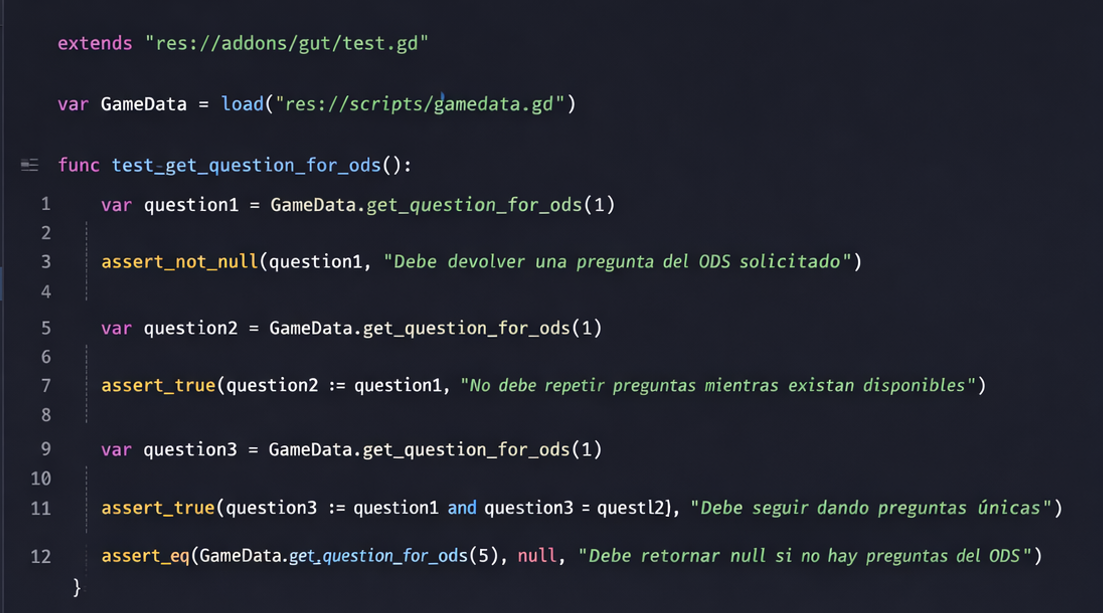
\includegraphics[width=0.9\textwidth]{Images/Caso de Prueba.png}
  \caption{Casos de prueba para la funcionalidad \texttt{get\_question\_for\_ods()} de la clase \texttt{GameData} (elaboración propia).\label{fig:casos_prueba_unitarias}}
\end{figure}

La figura anterior muestra la implementación de los casos de prueba utilizando el framework GUT, donde se definen ocho escenarios diferentes que evalúan si el sistema devuelve preguntas del ODS solicitado, evita repeticiones mientras existan preguntas disponibles y reinicia correctamente el ciclo cuando se agota el conjunto cargado desde el banco en formato JSON. La ejecución automatizada de estas pruebas permite verificar que la lógica implementada responde correctamente ante cada uno de los casos planteados, tal como se evidencia en los resultados presentados a continuación.

\begin{figure}[H]
  \centering
  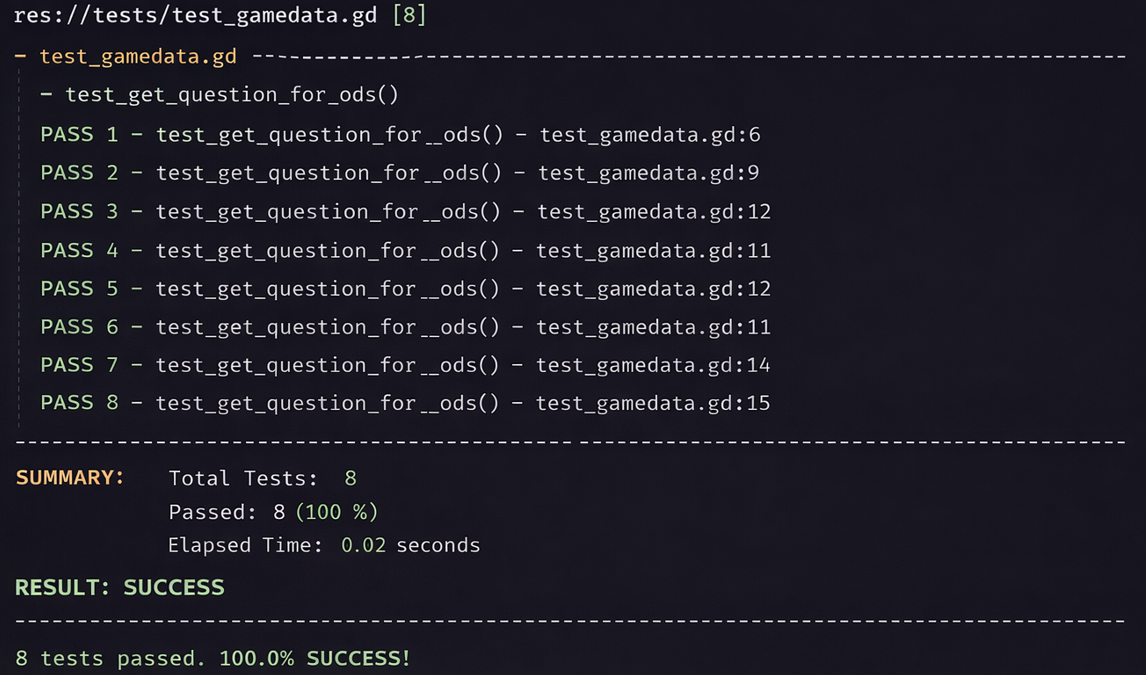
\includegraphics[width=0.6\textwidth]{Images/Resultado de Prueba.png}
  \caption{Resultado de pruebas para la clase \texttt{GameData} (elaboración propia).\label{fig:resultado_pruebas_unitarias}}
\end{figure}

Todas las funcionalidades probadas de esta forma pasaron las pruebas exitosamente, lo que no significa que no puedan existir defectos, ya que la interoperabilidad entre módulos puede causar problemas, lo que lleva a la necesidad de la aplicación de otro nivel de pruebas.

\subsection{Aplicación de pruebas de aceptación}
\label{subsec:aplicacion_pruebas_aceptacion}

Las pruebas de aceptación se realizaron siguiendo la metodología Extreme Programming, ejecutándose al finalizar cada una de las cinco iteraciones de desarrollo establecidas en el Capítulo 2. Esta organización permite validar incrementalmente el software conforme se implementan nuevas funcionalidades, detectando errores de forma temprana y asegurando que cada entrega parcial cumpla con los criterios de aceptación antes de proceder a la siguiente iteración.

Se ejecutaron un total de 18 casos de prueba vinculados a las historias de usuario implementadas para validar el cumplimiento de los criterios de aceptación establecidos. A continuación se presenta el caso de prueba correspondiente a la historia de usuario 9, que fue el único que presentó una no conformidad durante la Iteración 3. Los 17 casos de prueba restantes se encuentran detallados en el Anexo D.

\begin{table}[H]
\centering
\caption{Caso de prueba de aceptación \#9 Mostrar pregunta ODS (elaboración propia)\label{tab:cpa9}}
\renewcommand{\arraystretch}{1.3}
\begin{tabular}{|p{0.35\textwidth}|p{0.55\textwidth}|}
\hline
\multicolumn{2}{|c|}{\textbf{Caso de Prueba de Aceptación}} \\
\hline
\textbf{Código:} HU\#9\_PA\#1 & \textbf{Historia de Usuario:} 9 \\
\hline
\multicolumn{2}{|l|}{\textbf{Nombre:} Mostrar pregunta ODS} \\
\hline
\multicolumn{2}{|p{0.9\textwidth}|}{\textbf{Descripción:} Prueba realizada para verificar que al caer en una casilla ODS se muestre correctamente el panel de preguntas.} \\
\hline
\textbf{Pasos de ejecución:} & 1. Se mueve la ficha hasta una casilla ODS. \newline 2. Se verifica que aparezca el panel de preguntas. \newline 3. Se verifica que se muestren la pregunta y las opciones de respuesta. \\
\hline
\multicolumn{2}{|c|}{\textbf{Resultado:} No satisfactorio} \\
\hline
\end{tabular}
\end{table}

\subsubsection{Resultados de las pruebas de aceptación}

En las pruebas de aceptación se realizaron un total de 18 casos de prueba distribuidos en cinco iteraciones, obteniendo resultados mayormente positivos que evidencian la atención a los detalles críticos y la prevención de errores durante el proceso de implementación.

Los casos de prueba aplicados a las Iteraciones 1, 2, 4 y 5 dieron como resultado un 100\% de aprobación y 0\% de no conformidades, validando satisfactoriamente las funcionalidades base del videojuego, las mecánicas básicas de juego, las funcionalidades de cierre y las características complementarias. Sin embargo, en la Iteración 3 se detectó una no conformidad en el caso de prueba correspondiente a la historia de usuario 9 (Mostrar pregunta ODS), dando como resultado un 66.67\% de satisfacción y 33.33\% de insatisfacción para dicha iteración.

La no conformidad identificada consistió en un error de visualización en el panel de preguntas ODS, donde el texto de las opciones de respuesta se superponía con los bordes del panel cuando las respuestas contenían más de 50 caracteres, afectando la legibilidad y la experiencia de usuario. Este problema se presentaba específicamente en preguntas relacionadas con los ODS 8 (Trabajo decente y crecimiento económico) y ODS 16 (Paz, justicia e instituciones sólidas), cuyos enunciados tienden a ser más extensos.

Al corregir el error mediante el ajuste del tamaño de fuente y la implementación de saltos de línea automáticos en el componente de texto, y realizar nuevamente el caso de prueba a la historia de usuario 9, se obtuvo un resultado satisfactorio, elevando la Iteración 3 a un 100\% de aprobación. Tras esta corrección, se ejecutaron nuevamente todos los casos de prueba de las cinco iteraciones, confirmando que el videojuego \textit{Go Goals! Digital} cumple satisfactoriamente con todos los criterios de aceptación establecidos.

\subsection{Aplicación de pruebas de índice de aceptación}
\label{subsec:aplicacion_pruebas_indice}

Para la aplicación de esta prueba se contó con una muestra de diez jóvenes estudiantes de La Habana, con edades comprendidas entre 15 y 25 años, a los que se les distribuyó el videojuego \textit{Go Goals! Digital} para su evaluación. A dicha muestra se le administró un cuestionario estructurado, elaborado y diseñado específicamente para evaluar los criterios de aceptación.

\begin{table}[htbp]
\centering
\caption{Listado de estudiantes evaluadores (elaboración propia).\label{tab:probadores_beta}}
\renewcommand{\arraystretch}{1.3}
\begin{tabular}{|l|c|}
\hline
\textbf{Nombre y Apellidos} & \textbf{Edad} \\
\hline
José Miguel Martín Monzón & 18 \\
\hline
Oscar Raúl García Almestro & 22 \\
\hline
Royciel Chavez Garcés & 19 \\
\hline
Javier Ernesto Perdomo Batista & 24 \\
\hline
Yslen Marturelo Lorenzo & 16 \\
\hline
Janys Lourdes Cañizares de la Rosa & 21 \\
\hline
Pedro Luis Hernández Soto & 17 \\
\hline
Sofía Martínez Delgado & 25 \\
\hline
Carlos Alberto Ramos Pérez & 15 \\
\hline
Daniela Fernández Suárez & 20 \\
\hline
\end{tabular}
\end{table}

El cuestionario presentó la siguiente estructura:

\begin{longtable}{|p{0.95\textwidth}|}
\caption{Cuestionario de Satisfacción del Usuario -- Go Goals! Digital (elaboración propia).\label{tab:cuestionario_satisfaccion}} \\
\hline
\multicolumn{1}{|c|}{\textbf{Cuestionario de Satisfacción del Usuario -- Go Goals! Digital}} \\
\hline
\endfirsthead
\multicolumn{1}{c}
{{ \tablename\ \thetable{} -- Continuación de la página anterior}} \\
\hline
\multicolumn{1}{|c|}{\textbf{Cuestionario de Satisfacción del Usuario -- Go Goals! Digital}} \\
\hline
\endhead
\hline
\endfoot
\endlastfoot

\textbf{Instrucciones:} Por favor, responde cada pregunta considerando la siguiente escala de Likert:

1: Muy insatisfecho/a

2: Insatisfecho/a

3: Neutral

4: Satisfecho/a

5: Muy satisfecho/a \\
\hline
\multicolumn{1}{|c|}{\textbf{Sección 1: Experiencia General y Jugabilidad}} \\
\hline
\textbf{Jugabilidad General:}

¿Qué tan satisfecho/a estás con la jugabilidad general del videojuego? \\
\hline
\textbf{Control y Mecánicas:}

¿Qué tan intuitivas te resultan las mecánicas de control (lanzar dado, mover fichas, responder preguntas) en el juego? \\
\hline
\textbf{Desafíos y Equilibrio:}

¿Consideras que el nivel de desafío de las preguntas es adecuado para tu edad? \\
\hline
\multicolumn{1}{|c|}{\textbf{Sección 2: Interfaz y Diseño Visual}} \\
\hline
\textbf{Usabilidad e Interfaz:}

¿Qué tan clara e intuitiva es la interfaz del videojuego?

¿Qué tan útil te han resultado los tutoriales y elementos de ayuda integrados? \\
\hline
\textbf{Estética y Diseño Gráfico:}

¿Qué tan atractivo y coherente encuentras el diseño visual y la estética general del videojuego? \\
\hline
\multicolumn{1}{|c|}{\textbf{Sección 3: Rendimiento Técnico}} \\
\hline
\textbf{Rendimiento del Sistema:}

¿Estás satisfecho/a con el desempeño técnico del juego en términos de tiempos de carga, estabilidad y fluidez durante la experiencia de juego? \\
\hline
\multicolumn{1}{|c|}{\textbf{Sección 4: Contenido Educativo y Relación con los ODS}} \\
\hline
\textbf{Integración de Contenido Educativo:}

¿Qué tan claro y efectivo es el contenido relacionado con los Objetivos de Desarrollo Sostenible (ODS) dentro del videojuego? \\
\hline
\textbf{Impacto Educativo:}

¿Crees que el contenido del juego te ha motivado a informarte o reflexionar sobre temas de sostenibilidad? \\
\hline
\textbf{Balance entre Entretenimiento y Educación:}

¿Consideras que el juego logra un buen equilibrio entre ser entretenido y cumplir con su función educativa en cuanto a la promoción de los ODS? \\
\hline
\multicolumn{1}{|c|}{\textbf{Sección 5: Satisfacción Global y Recomendación}} \\
\hline
\textbf{Satisfacción Global:}

En general, ¿qué tan satisfecho/a estás con tu experiencia en \textit{Go Goals! Digital}? \\
\hline
\textbf{Recomendación:}

¿Recomendarías este videojuego a otras personas interesadas en videojuegos educativos o en sostenibilidad? (Opciones: Sí / No) \\
\hline
\end{longtable}

Al aplicarlo se obtuvieron resultados altamente positivos, con todos los usuarios recomendando probar el videojuego.
\begin{table}[H]
\centering
\caption{Resultados del cuestionario de satisfacción (elaboración propia).\label{tab:resultados_cuestionario}}
\renewcommand{\arraystretch}{1.3}
\begin{tabular}{|l|c|c|c|}
\hline
\textbf{Categoría} & \textbf{Respuestas positivas} & \textbf{Respuestas neutrales} & \textbf{Respuestas negativas} \\
\hline
Experiencia General y Jugabilidad & 30 & 0 & 0 \\
\hline
Interfaz y Diseño Visual & 28 & 2 & 0 \\
\hline
Rendimiento Técnico & 10 & 0 & 0 \\
\hline
Contenido Educativo y ODS & 30 & 0 & 0 \\
\hline
Satisfacción Global & 10 & 0 & 0 \\
\hline
\textbf{Total} & \textbf{108} & \textbf{2} & \textbf{0} \\
\hline
\end{tabular}
\end{table}

Tomando estos resultados se aplica la fórmula del CSAT, donde se divide el número de respuestas positivas entre el total de respuestas y se multiplica por 100. Al aplicar esta métrica se obtiene un cociente de 108 respuestas positivas dividido entre 110 respuestas totales que, al ser multiplicado por 100, resulta en 98.18\%. Este valor se considera extremadamente alto y valida objetivamente la calidad técnica, el diseño instruccional y la aceptación del videojuego educativo \textit{Go Goals! Digital} por parte de su público objetivo.

%---------------------------------------------------------------------------
\section*{Conclusiones del capítulo}

El diseño estructurado de la validación permitió asegurar una alta calidad en el proceso evaluativo, siguiendo las buenas prácticas de la metodología Extreme Programming. A través de la aplicación de pruebas unitarias automatizadas se garantizó el correcto funcionamiento de los módulos lógicos internos sin dependencias externas, previniendo defectos de integración. Las pruebas de aceptación validaron el videojuego en su totalidad desde la perspectiva de los usuarios finales. Finalmente, el índice de aceptación del 98.18\% documentado mediante el instrumento CSAT confirma que \textit{Go Goals! Digital} cumple satisfactoriamente con los objetivos pedagógicos y lúdicos planteados, resultando en un producto tecnológico altamente valorado por su público objetivo.
